\usetikzlibrary{positioning}

\begin{document}

\def\title{Worksheet 5}

\newcommand{\qitem}{\qpart\item}

\renewcommand{\labelenumi}{(\alph{enumi})} % change default enum format to (a)
\renewcommand{\theenumi}{(\alph{enumi})} % fix reference format accordingly.
\renewcommand{\labelenumii}{\roman{enumii}.} % second level labels.
\renewcommand{\theenumii}{\roman{enumii}.}

\maketitle

\vspace{0.5em}

\begin{qunlist}
% Authors: Son Tran, Naomi Sagan, Taejin Hwang
% Emails: sontran@berkeley.edu, naomi.sagan@berkeley.edu, taejin@berkeley.edu

\qns{Change of Coordinates}

Many engineering problems can be difficult to solve in its standard xyz coordinates, but may be much easier in a different coordinate system.
In this set, we will review the process of \textbf{change of basis} between coordinate systems.
Remember that a \emph{change of basis} can be represented by a invertible, square matrix. \vskip 1pt
Let's first start with an example:
Consider the vector $\vec{x} = \begin{bmatrix} x_1 \\ x_2 \end{bmatrix}.$ 
When we write a vector in this form, we are implicitly representing it with the \textbf{standard basis} for $\R^{2}$, $\vec{e_1} = \begin{bmatrix} 1 \\ 0 \end{bmatrix}$ and $\vec{e_2} = \begin{bmatrix} 0 \\ 1 \end{bmatrix}.$ \vspace{1em} 
This means that we can write $\vec{x}$ as a linear combination using standard basis vectors $\vec{x} = x_1\vec{e_1} + x_2\vec{e_2}$. \vspace {1em} 
Now, what if we want to represent $\vec{x}$ as a linear combination of another set of basis vectors, say $\vec{v_1} = \begin{bmatrix} 1 \\ 1 \end{bmatrix}$ and $\vec{v_2} = \begin{bmatrix} 0 \\ -1 \end{bmatrix}?$ \vskip 1pt
This means that we need to find scalars $\alpha_{1}$ and $\alpha_{2}$ such that $\vec{x} = \alpha_1 \vec{v_1} + \alpha_2 \vec{v_2}$.
We can write this equation in matrix form:
\[
  \begin{bmatrix}
    | & | \\
    \vec{v_1} & \vec{v_2} \\
    | & |
  \end{bmatrix}
  \begin{bmatrix} \alpha_1 \\ \alpha_2 \end{bmatrix} = \begin{bmatrix} x_1 \\ x_2 \end{bmatrix}
.\]

Or equivalently:
\[
  \begin{bmatrix}
    1 & 0 \\
    1 & -1
  \end{bmatrix}
  \begin{bmatrix} \alpha_1 \\ \alpha_2 \end{bmatrix} = \begin{bmatrix} x_1 \\ x_2 \end{bmatrix}
.\]
Thus we can find $\alpha_1$ and $\alpha_2$ by solving a system of linear equations as seen in 16A. \\
These scalars $\alpha_1$ and $\alpha_2$ are called the coordinates of $\vec{x}$ \textbf{in the basis} $V = \{\vec{v_1}, \vec{v_2} \}.$

For the following problems, we will look at a vector $\vec{x}$ currently in the standard basis 
and its representation in a different basis: $V = \{\vec{v_1}, \vec{v_2} \}.$ \vskip 4pt
We will refer to the vector $\vec{x}$ using coordinates from the basis $V$ as $[\vec{x}]_V$. In other words, \vskip 3pt 
if $\vec{x} = \begin{bmatrix} x_1 \\ x_2 \end{bmatrix},$ and $[\vec{x}]_V = \begin{bmatrix} \alpha_1 \\ \alpha_2 \end{bmatrix},$ then $\vec{x} = x_1 \vec{e_1} + x_2 \vec{e_2}$ or $\vec{x} = \alpha_1 \vec{v_1} + \alpha_2 \vec{v_2}.$

\begin{enumerate}
  % Part(a)
  \qitem Now let's say we have a vector that is originally using coordinates from the basis $V$. 
  That is $[\vec{x}]_V = \begin{bmatrix} 3 \\ 3 \end{bmatrix}.$ We are told that the basis $V$ is:
  \begin{gather*}
    \vec{v_1} =
    \begin{bmatrix}
      1 \\
      1
    \end{bmatrix},
    \vec{v_2} = \begin{bmatrix}
      1 \\
      -1
    \end{bmatrix}
  \end{gather*}
  What equation gives the coordinates of $\vec{x}$ in the standard basis?

  % Part(a) solution
  \sol{
    Since the vector $\vec{x}$ is currently written in coordinates using the basis, $V = \{\vec{v_1}, \vec{v_2} \},$
    we know that $\vec{x} = 3 \begin{bmatrix} 1 \\ 1 \end{bmatrix} + 3 \begin{bmatrix} 1 \\ -1 \end{bmatrix} = V [\vec{x}]_V$
    where $V$ is the matrix $\begin{bmatrix} 1 & 1 \\ 1 & -1 \end{bmatrix}.$ Therefore,
    $$
    \vec{x} =
    \begin{bmatrix}
      1 & 1 \\
      1 & -1
    \end{bmatrix}
    \begin{bmatrix}
      3 \\
      3
    \end{bmatrix}
    $$
  }

  % Part(b)
  \qitem Let $\vec{v}_1, \vec{v}_2$ be the same as above.
  Let $\vec{x} = \begin{bmatrix} 2 \\ -1 \end{bmatrix}$ in the standard basis.
  Give the coordinates of $\vec{x}$ in the basis $V$.
  What equation gives the coordinates of $\vec{v}$ in the standard basis?

  % Part(b) solution
  \sol {
    If we denote the vector in the new basis as $[\vec{x}]_V = \begin{bmatrix} \alpha_1 \\ \alpha_2 \end{bmatrix}$, then we can write out the following equation: $\vec{x} = \alpha_1 \vec{v_1} + \alpha_2 \vec{v_2} = V [\vec{x}]_V$ where $V$ is the same matrix used in the previous part.
    Then it follows that $[\vec{x}]_V = V^{-1} \vec{x}.$
    This can be solved numerically to get the vector
    \begin{equation*}
      [\vec{x}]_V =
      \frac{1}{2} \begin{bmatrix}
        1 \\
        3
      \end{bmatrix}
    \end{equation*}
  }

  \end{enumerate}

  Now that we've had some mechanical practice, we'll look at the representation of linear operators through different bases. 
  For a linear transformation, we can represent the input-output relationship with the matrix vector equation:
  $\vec{y} = A \vec{x}$ where $\vec{x}$ is the input, and $\vec{y}$ is the output vector.
  In this question we will look at how the linear operator represented by the matrix $A$ looks in a \textit{different basis} $V$.
  Remember that the vector $\vec{x}$ is implicitly written in the \textbf{standard basis} while the vector $[\vec{x}]_V$ is a vector using coordinates from the \textbf{V-basis.}

  \begin{enumerate}[resume]
  %part c
  \qitem Let $[\vec{x}]_V$ be a vector using $V$ coordinates, and $V$ be a change of coordinates matrix from the $V$ basis to the standard basis. \\
  How can we represent $[\vec{x}]_V$ in terms kf $\vec{x}$ and $V?$
  \sol {
    We are given a matrix $V$ that converts $V$ coordinates to standard coordinates. 
    This means that $V^{-1}$ will be the matrix that converts standard coordinates to the $V$ coordinates.
    Therefore, in order to get $[\vec{x}]_V$ we multiply $V^{-1}$ with $\vec{x},$ to get
    $V^{-1} \vec{x} = [\vec{x}]_V$.
  }

  % Part(d)
  \qitem Now suppose we have another basis $R = \{w_1, .. , w_n\}$ and the change of basis from $R$ to $V$ is represented by the matrix $W.$ This means that if we have a vector $[\vec{x}]_R$ in R-coordinates, to get the coordinate representation in V-coordinates, $[\vec{x}]_V = W[\vec{x}]_R.$ What would the change of basis matrix that takes a vector in $R$ coordinates and outputs a vector in standard coordinates look like?
  \sol {
    We want to get represent the vector $\vec{x}$ in standard coordinates.
    We are looking for a matrix $U$ such that
    $$\vec{x} = U [\vec{x}]_R.$$
    We currently know that in order to go from V-coordinates to standard, we must multiply by the matrix $V$.
    $$\vec{x} = V [\vec{x}]_V$$.
    We also know that to go from R-coordinates to V-coordinates, we must multiply by the matrix $W.$
    $$[\vec{x}]_V = W [\vec{x}]_R.$$
    Therefore, by substituting $[\vec{x}]_V,$ we see that
    $$\vec{x} = V W [\vec{x}]_R.$$
    It follows that the matrix $U = VW.$
  }

  % % Part(d)
  % \qitem Now let $B$ be a linear operator in $\beta$ coordinates. This means that it will take in a vector $[\vec{x}]_\beta$ as an input and output $[\vec{y}]_\beta.$ Given a vector $\vec{x}$ in standard coordinates, why can't we multiply $B \vec{x}$ to get the output $\vec{y}$ in standard coordinates?

  % \sol{
  %   The transformation $B$ "lives" in a different world. It can only accept vectors in $\beta$ coordinates as inputs. 
  %   Therefore, in order to solve this, we must convert $\vec{x}$ into $\beta$ coordinates.
  % }

  % Part(e)
  \qitem Now let $B$ be a linear operator in $V$ coordinates.
  This means that it will take in a vector $[\vec{x}]_V$ as an input and output $[\vec{y}]_V$.
  Then if $\vec{y} = A \vec{x}$, what is $A$ in the standard basis?

  \sol {
    There will be two main issues we need to address in this question. First off, we need a $V$ coordinate input. Secondly, the output of the $B$ matrix is in $V$ coordinates, and we will need to convert that back to standard coordinates. 

    Therefore, we take the following steps.

    \begin{enumerate}
      \item Let's first make our input into $B$ in $V$ coordinates. 
      $$\text{Let } V [\vec{x}]_V = \vec{x}.$$
      \item Now if we input $[\vec{x}]_V$ we will get some output:
      $$\vec{w} = B [\vec{x}]_V.$$
      \item However, $\vec{w}$ is in $V$ coordinates, so we must convert back to standard coordinates using $V^{-1}.$
      $$V^{-1} [\vec{x}]_V =  \vec{w}$$
      \item Cascading all of our matrix multiplications, we end up with:
      $$\vec{y} = V B V^{-1} \vec{x}.$$
    \end{enumerate}
    Therefore, we can see that $A = V B V^{-1} .$

    The following can also be represented in this state diagram: 

    Note that when cascading transformations, we apply them to the \textbf{left} of the existing transformation.

    \begin{figure}[H]
      \centering
      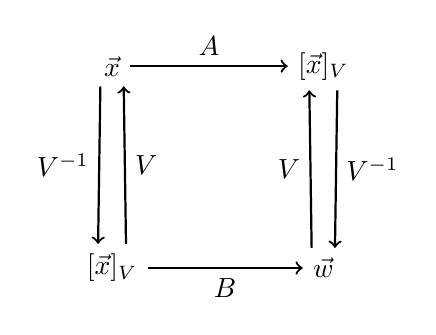
\begin{tikzpicture}[node distance = 2cm, thick]%
        \node (1) {$\vec{x}$};
        \node (2) [right=of 1] {$[\vec{x}]_V$};
        \node (3) [below=of 2] {$\vec{w}$};
        \node (4) [below=of 1] {$[\vec{x}]_V$};
        \draw[->] (1) -- node [midway,above] {$A$} (2);
        \draw[->] (1.240) -- node [midway,left]{$V^{-1}$} (4.120);
        \draw[->] (4.60) -- node [midway,right]{$V$} (1.300);
        \draw[->] (2.300) -- node [midway,right]{$V^{-1}$} (3.60);
        \draw[->] (3.120) -- node [midway,left]{$V$} (2.240);
        \draw[->] (4) -- node [midway,below] {$B$} (3);
      \end{tikzpicture}%
    \end{figure}
  }
  % % Part(c) solution
  % \sol{
  %   Start by writing $\vec{x_1}$ in terms of $\vec{z_1}$:
  %   $$ \vec{x_1} = V \vec{z_1} $$
  %   Then, apply the transformation $A$ to $\vec{x_1}$, substituting $V \vec{z_1}$ for $\vec{x_1}$:
  %   $$ \vec{x_2} = A V \vec{x_1} $$
  %   Finally, left-multiply both sides by $V^{-1}$ to change $\vec{x_2}$ to the eigenbasis:
  %   $$ \vec{z_2} = V^{-1} \vec{x_2} = V^{-1} A V \vec{z_1} $$

  %   $$A' = V^{-1} A V =
  %   \begin{bmatrix}
  %     1 & 1 \\
  %     -2 & 1
  %   \end{bmatrix}^{-1}
  %   \begin{bmatrix}
  %     3 & -1 \\
  %     -2 & 4
  %   \end{bmatrix}
  %   \begin{bmatrix}
  %     1 & 1 \\
  %     -2 & 1
  %   \end{bmatrix}
  %   $$

  %   $A'$ represents the transformation $A$ in the eigenbasis of $A$, so we know that $A'$ is the diagonal matrix:
  %   $$ A' =
  %   \begin{bmatrix}
  %     \lambda_1 & 0 \\
  %     0 & \lambda_2
  %   \end{bmatrix} =
  %   \begin{bmatrix}
  %     5 & 0 \\
  %     0 & 2
  %   \end{bmatrix} $$

  %   In general, suppose we have a linear transformation $T$ represented by a $n \times n$ matrix that transforms $\vec{u} \in \R^{n}$ to $\vec{v} \in \R^{n}$:
  %   \[
  %     \vec{v} = T\vec{u}
  %   .\]
  %   Suppose we have a basis vectors $\vec{a_1}, \cdots, \vec{a_n} \in \R^{n}$, and the vectors $\vec{u}, \vec{v}$ above are represented in this basis:
  %   \[
  %     \begin{aligned}
  %       \vec{u_a} &= u_{a_1}\vec{a_1} + \cdots + u_{a_n}\vec{a_n} \\
  %       \vec{v_a} &= v_{a_1}\vec{a_1} + \cdots + v_{a_n}\vec{a_n}.
  %     \end{aligned}
  %   \]
  %   Thus we have
  %   \[
  %     \begin{aligned}
  %       T\vec{u}          &= \vec{v} \\
  %       TA\vec{u_a}       &= A\vec{v_a} \\
  %       A^{-1}TA\vec{u_a} &= \vec{v_a}.
  %     \end{aligned}
  %   \]
  %   By pattern matching, we see that if we set $T_a = A^{-1}TA$, we get the relationship $T_a\vec{u_a} = \vec{v_a}$ in the new basis.
  %   The correspondences stated above are all represented in the following diagram:
  %   % \begin{figure}[H]
  %   %   \centering
  %   %   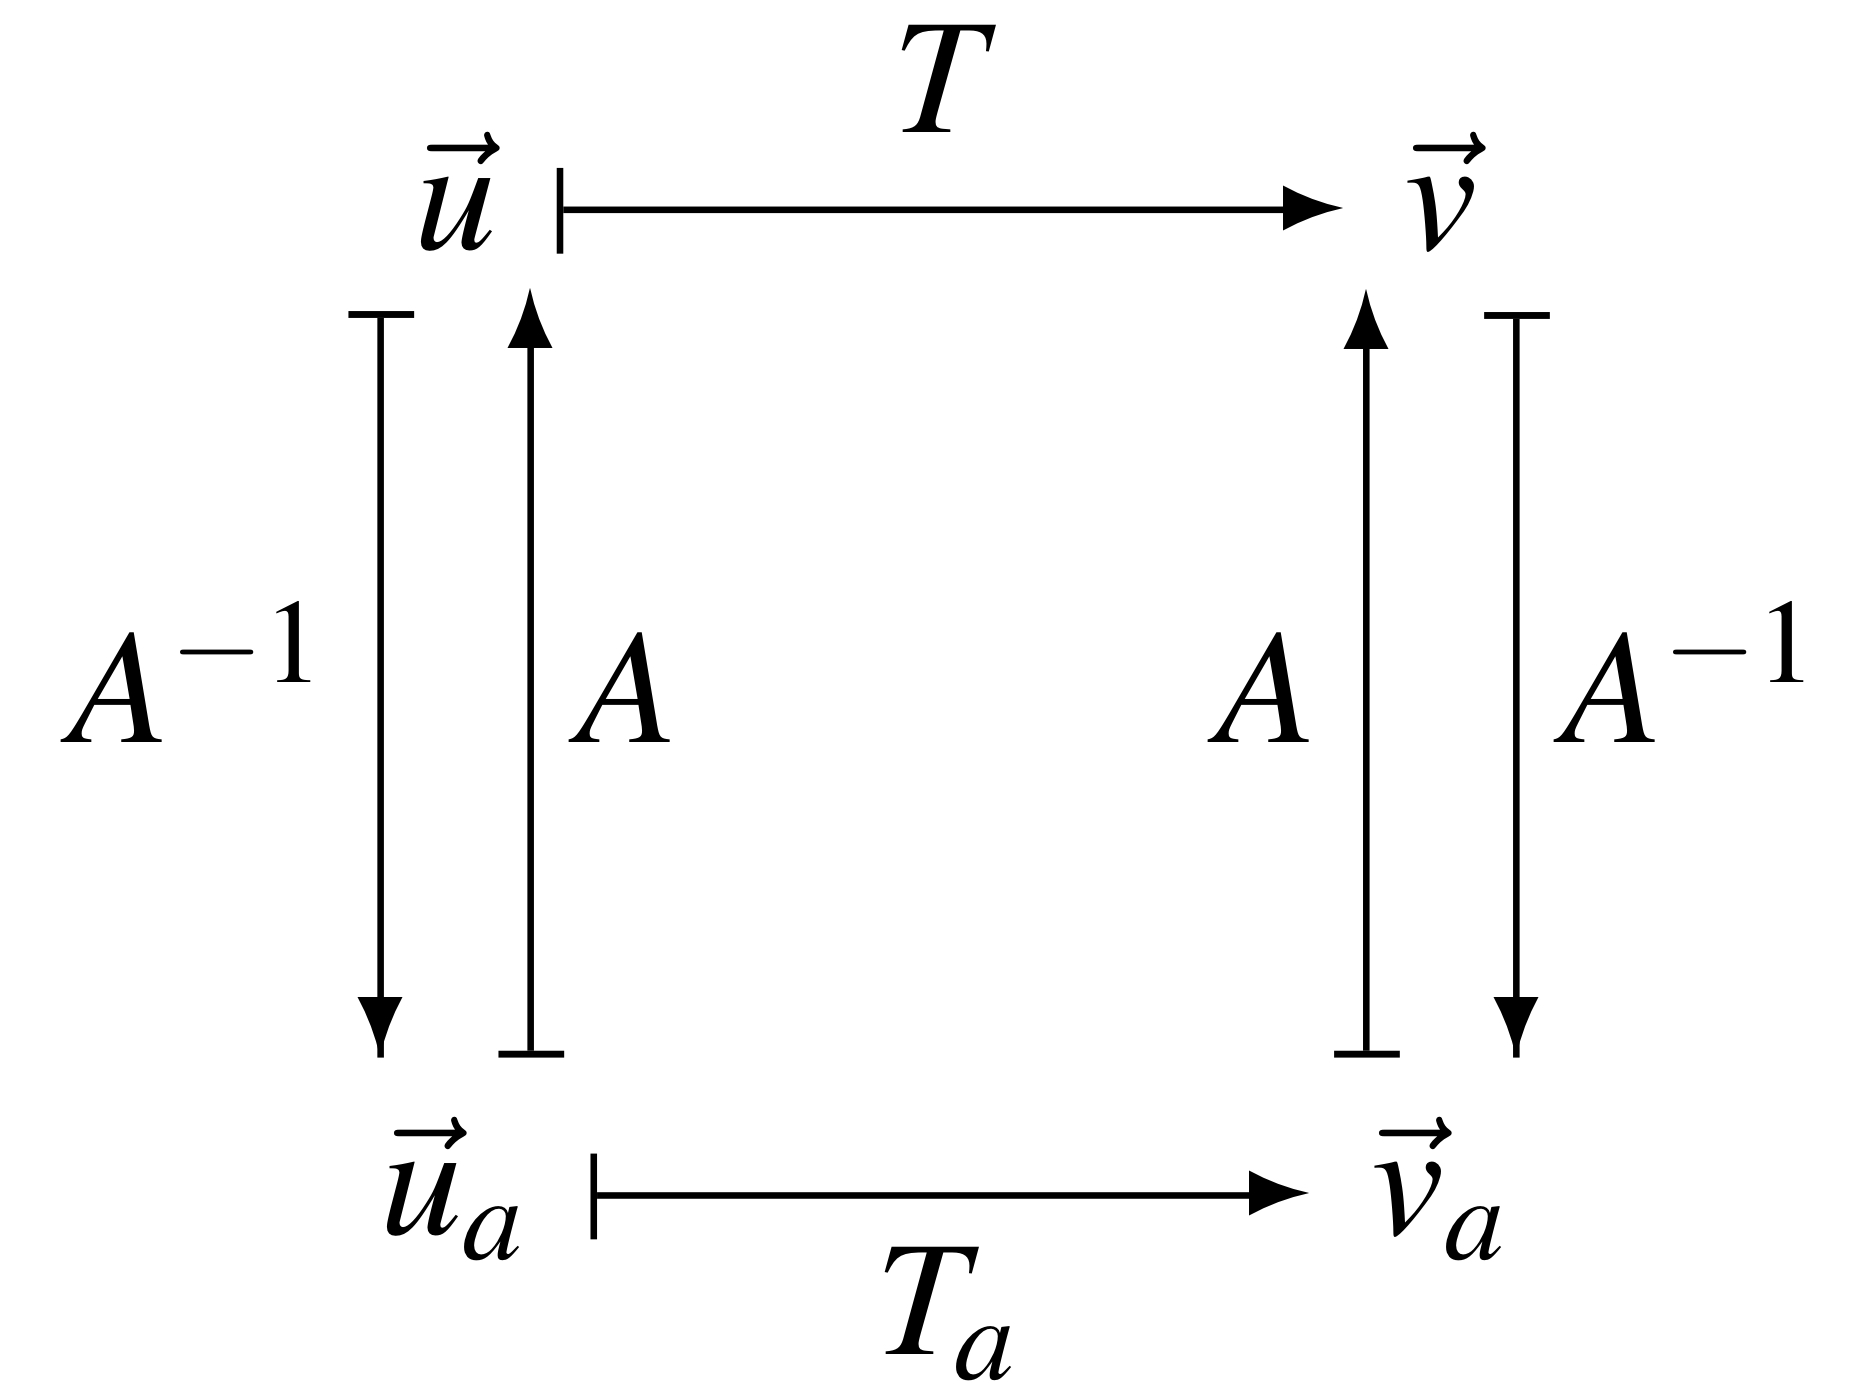
\includegraphics[scale=0.1]{\bank/statespace/figures/change_of_basis.jpg}
  %   % \end{figure}
\end{enumerate}

\newpage
% Authors: Tony Li, and authors of diagonalization.tex
% Email: songli@berkeley.edu

\qns{Diagonalization and Diagonalizability}

\textbf{Diagonal matrices}, matrices where all entries outside of the diagonal are zero.
Diagonal matrices come handy in terms of solving systems of linear equations, solving for vector case of differential equations, finding out the determinant, etc. 
\newline \textbf{Diagonalization} is a procedure that we transform a matrix $A$ into three matrices multiplied together, whihc means 
$A=V{\Lambda}V^{-1}$, where $V^{-1}$ is the inverse of $V$, and $\Lambda$ is a diagonal matrix.

In this problem, we'll investigate what $V$ and $\Lambda$ truly are.

\begin{enumerate}

\qitem First we need to recall some pretty useful concepts, eigenvalues and eigenvectors. For a matrix $A$, if we can write the
equation that $A\vec{v}=\lambda\vec{v}$, where $\lambda$ is non-zero and $\vec{v}$ is non-zero vector, then we say that $\vec{v}$ and $\lambda$ is a pair of eigenvector and eigenvalue of $A$.
Given that 
$$A = \begin{bmatrix}
  2 & 2 \\
  5 & -1
  \end{bmatrix}$$
\textbf{Can you explain why $A$ has two eigenvalues and in a more general case, how many eigenvalues does a n by n matrix have?}
\ws{
\vspace{30px}
}

\meta{
  Introduce how we solve for eigenvalues and eigenvectors.
}

\sol{
  Based on the definition, we know $A\vec{v}=\lambda\vec{v}$, then we can write it into another form, $(A-{\lambda}I_n)\vec{v}=0$, where $I_n$
  is the identity matrix. As a result, since $\vec{v}$ can not be a zero vector, $(A-{\lambda}I_n)\vec{v}=0$ is a homogenous linear system solving for $\vec{v}$.
  $\vec{v}$ has non zero solution, only when $A-{\lambda}I_n$ is not invertible, which implies that $det(A-{\lambda}I_n)=0$.
  Solving a $det(A-{\lambda}I_n)=0$ is essentially solving a polynomial with degree n, so \textbf{$\lambda$ should have n solutions}.
  Plase note that, $\lambda$'s could be complex numbers.
}

\qitem \textbf{Find eigenvalues ${\lambda}_1$ and ${\lambda}_2$ and their corresponding eigenvectors $\vec{v_1}$ and $\vec{v_2}$}, where ${\lambda}_1\le{\lambda}_2$,
and both of the eigenvectors have length 1.

\ws{
\vspace{100px}
}

\sol{
  $$det(A-{\lambda}I_n)=det(\begin{bmatrix}
    2-\lambda & 2\\
    5 & -1-\lambda
  \end{bmatrix})=(2-\lambda)(-1-\lambda)-2\times5={\lambda}^2-\lambda-12=0$$
  \newline After solving the quadratic equation above, We have ${\lambda}_1=-3$ and ${\lambda}_2=4$.
  Let's plug two eigenvalues into $(A-{\lambda}I_n)\vec{v}=0$.
  $$\begin{bmatrix}
    2-{\lambda}_1 & 2\\
    5 & -1-{\lambda}_1 
  \end{bmatrix}\vec{v_1} = \begin{bmatrix}
    5 & 2\\
    5 & 2
  \end{bmatrix}\vec{v_1}=0$$
  $$\Rightarrow \vec{v_1}=\begin{bmatrix}
    2C\\
    -5C\\
  \end{bmatrix}, C\in\mathbb{R}$$
  Since $\vec{v_1}$ has length 1, then $$\vec{v_1}=\begin{bmatrix}
    \frac{2}{\sqrt{29}}\\
    \frac{-5}{\sqrt{29}}
  \end{bmatrix}$$
  \newline Similarly, we would have 
  $$\vec{v_2}=\begin{bmatrix}
    \frac{1}{\sqrt{2}}\\
    \frac{1}{\sqrt{2}}
  \end{bmatrix}$$
}

\end{enumerate}

With the eigenvectors $\vec{v_1}$ and $\vec{v_2}$, define $V$ to be the matrix:
$$V = \begin{bmatrix}
\vec{v_1} & \vec{v_2}
\end{bmatrix}$$
Columns of this matrix $V$ are called eigenbasis of $A$.
With the eigenvalues ${\lambda}_1$ and ${\lambda}_2$, define $\Lambda$ to be the matrix:
$$\Lambda = \begin{bmatrix}
  {\lambda}_1 & 0\\
  0 & {\lambda}_2
  \end{bmatrix}$$
\begin{enumerate}[resume]
\qitem Now, we need to \textbf{prove that $A=V{\Lambda}V^{-1}$}. Assume that $V$ is invertible.
\newline \emph{Hint:}First, transform the above equation into the form $AV=V{\Lambda}$. Then, expand $V$ and $\Lambda$ with
matrices provided above.
\ws{\vspace{100px}}

\meta{
  Show students that the procedure in the solution is applicable to prove $A=V{\Lambda}V^{-1}$, even if A is n by n.
}

\sol{
  Based on the definition of eigenvalues and eigenvectors, let $\vec{v_1}$, $\vec{v_2}$,..., $\vec{v_n}$ be n eigenvectors
  of the n by n matrix $A$, and their corresponding eigenvalues are ${\lambda}_1$, ${\lambda}_2$,..., ${\lambda}_n$.
  Now, we have $V=[\vec{v_1}, \vec{v_2}, ..., \vec{v_n}]$.
  $$AV=A[\vec{v_1}, \vec{v_2}, ..., \vec{v_n}]=[A\vec{v_1}, A\vec{v_2}, ..., A\vec{v_n}]=[{\lambda}_1\vec{v_1}, {\lambda}_2\vec{v_2}, ..., {\lambda}_n\vec{v_n}]$$
  $$=[\vec{v_1}, \vec{v_2}, ..., \vec{v_n}]\begin{bmatrix}
    {\lambda}_1&0&0&...\\
    0&{\lambda}_2&0&...\\
    ...&...&...&...\\
    0&0&...&{\lambda}_n
  \end{bmatrix}=V\Lambda$$
}
\qitem Now you know that in order to diagonalize a given matrix, we need to calculate eigenvalues and eigenvectors first. However, there is still a premise we need to deal with: \textbf{when is a matrix diagonalizable?
If a matrix is diagonalizable, does it imply that the matrix is also invertible? In the opposite direction, is an invertible matrix always diagonalizable?}
\ws{\vspace{40px}}

\meta{
  The essence of this question is to tell students that invertibility does not work here, and most students would tend to use invertibility
  to explain diagonalizability.
}

\sol {
  If we look at the steps of proving $A=V{\Lambda}V^{-1}$, we made assumption that proving $A=V{\Lambda}V^{-1}$ is equivalent to
  proving $AV=V\Lambda$. The only difference here is whether $V$, or the eigenbasis, is invertible. Therefore, if a matrix is diagonalizable,
  its eigenbasis should have n linearly independent eigenvectors, or the eigenbasis is invertible, or the determinant of eigenbasis is not 0.
  \newline The invertibility of the matrix itself does not imply its diagonalizability, and the diagonalizability also does not imply invertibility.
  \newline Counterexample of the first claim: 
  $$M=\begin{bmatrix}
    1&1\\
    0&1
  \end{bmatrix}$$
  Here, $M$ is invertible since $det(M)\ne0$, but it have two equal-value eigenvalues 1, which means that two eigenvectors can not be not
  linearly independent, so it is not diagonalizable.
  \newline Counterexample of the second claim:
  $$N=\begin{bmatrix}
    0&0\\
    0&1
  \end{bmatrix}$$
  In this case, $N$ is diagonalizable, since it has two distinct eigenvalues ${\lambda}_1=0$ and ${\lambda}_2=1$. Eigenvectors corresponding to distinct eigenvalues are linearly independent.
  However, $N$ is not invertible, because $det(N)=0$.
}
\end{enumerate}
Let's now concentrate on the diagonalization with help of change of basis. We'll explore the diagonalization more clearly from the
perspective of change of basis.
\begin{enumerate}[resume]

\qitem Let $\widetilde{\vec{x}}$ be the coordinates of $\vec{x}$ in the eigenbasis. 
This means that for some arbitrary vector represented in the eigenbasis $\widetilde{\vec{x}} = \begin{bmatrix} \alpha_1 \\ \alpha_2 \end{bmatrix}$, 
the corresponding representation in standard coordinates is a linear combination of the columns of $V$: $\vec{x} = \alpha_1 \vec{v_1} + \alpha_2 \vec{v_2}$. \textbf{What is $\widetilde{\vec{x}}$ in terms of $V$ and $\vec{x}?$}

(\textit{Hint: Write $\vec{x}$ in terms of $V$ and $\tilde{\vec{x}}$, then go from there.})

\ws{\vspace{3em}}

\meta{
  The line $\alpha_1 \vec{v_1} + \alpha_2 \vec{v_2} = V \widetilde{\vec{x}}$ is not the most intuitive.
  It may require you showing on the board, why matrix vector multiplication can be seen as a linear combination of the columns.
}

\sol{
  $\vec{x} = \alpha_1 \vec{v_1} + \alpha_2 \vec{v_2} = V \widetilde{\vec{x}}.$ So it follows that $\widetilde{\vec{x}} = V^{-1} \vec{x}.$
}

\qitem It is often helpful to visualize the change of basis in a state diagram, where \textit{each arrow represents left-multiplying the variable it's coming out of by the corresponding matrix.} \textbf{Fill in the missing matrix operations in the state diagram based on your answer from the previous part.}

\ws {
  \begin{figure}[H]
    \centering
    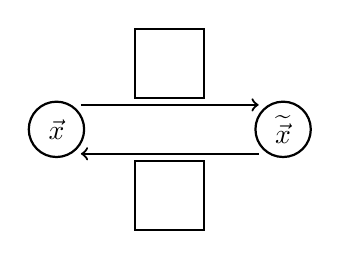
\begin{tikzpicture}[node distance = 2cm, thick,every node/.style={inner sep=0.25em,outer sep=0.25em}]%
      \node (1) [circle,draw,minimum size=2em] {$\vec{x}$};
      \node (2) [circle,draw,right=of 1,minimum size=2em] {$\widetilde{\vec{x}}$};
      \draw[->] (1.45) -- node [rectangle,draw,midway,above,minimum size=2.5em] {} (2.135);
      \draw[->] (2.225) -- node [rectangle,draw,midway,below,minimum size=2.5em] {} (1.315);
    \end{tikzpicture}%
  \end{figure}
}

\meta {
  Not everyone finds this diagram the most intuitive, but it definitely helps a large percentage of students. Stress to students that it's always better to understand the intuitive meaning behind change of basis than to remember any particular change of basis formula. This intuitive meaning is bridging between coordinate systems, which can be visualized with this diagram.
}

\sol {
  \begin{figure}[H]
  \centering
  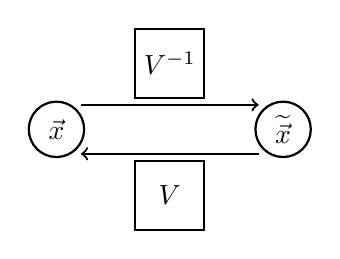
\begin{tikzpicture}[node distance = 2cm, thick,every node/.style={inner sep=0.25em,outer sep=0.25em}]%
    \node (1) [circle,draw,minimum size=2em] {$\vec{x}$};
    \node (2) [circle,draw,right=of 1,minimum size=2em] {$\widetilde{\vec{x}}$};
    \draw[->] (1.45) -- node [rectangle,draw,midway,above,minimum size=2.5em] {$V^{-1}$} (2.135);
    \draw[->] (2.225) -- node [rectangle,draw,midway,below,minimum size=2.5em] {$V$} (1.315);
  \end{tikzpicture}%
  \end{figure}
}


\qitem Now that we are able to switch back and forth between the coordinate systems, let's see how the linear transformation brought by $A$ can be viewed as a diagonal scaling transformation in the eigenbasis coordinate system.% Might be a bit confusing.

Let $\vec{y} = A \vec{x}$, and $\vec{x} = \alpha_1 \vec{v_1} + \alpha_2 \vec{v_2}$, using the same matrix $A$ and eigenvectors $\vec{v_1}, \vec{v_2}$ from before. Let $\widetilde{\vec{x}}$, $\widetilde{\vec{y}}$ be the coordinates of $\vec{x}$, $\vec{y}$ in the eigenbasis. \textbf{Find $\widetilde{\vec{x}}$ and $\widetilde{\vec{y}}$ in terms of $\alpha_1, \alpha_2, \lambda_1, \lambda_2$. What can we say about the relationship between $\widetilde{\vec{x}}$ and $\widetilde{\vec{y}}$?} % Might be confusing as to what the problem is asking compared to the next part.

(\textit{Hint}: Your answers shouldn't be in terms of the original $\vec{x}$ or $\vec{y}$.
 Use what you know about the coordinates of a vector in a certain basis; there is no need to invert any matrices or do any major computation.)

\ws {
  \vspace{200px}
}

\meta {
  Students may try to use what they found in the previous parts to multiply the vectors by $V^{-1}$. While this is technically right, make sure they understand what exactly
  that transformation is doing and why they don't need to do any matrix computation to find the coordinates of $\vec{y}$ in the eigenbasis.
}

\sol {
  $$\widetilde{\vec{x}} = \begin{bmatrix} \alpha_1 \\ \alpha_2 \end{bmatrix}$$

  \begin{align*}
    \vec{y} &= A \vec{x} \\
    &= A(\alpha_1 \vec{v_1} + \alpha_2 \vec{v_2}) \\
    &= \alpha_1 A \vec{v_1} + \alpha_2 A \vec{v_2} \\
    &= \alpha_1 \lambda_1 \vec{v_1} + \alpha_2 \lambda_2 \vec{v_2} \\
    \implies \widetilde{\vec{y}} &= \begin{bmatrix} \alpha_1 \lambda_1 \\ \alpha_2 \lambda_2 \end{bmatrix}
  \end{align*}

  This means that the matrix $D$ relating the two coordinates in the eigenbasis must be a diagonal scaling transformation, with the eigenvalues as the amount each dimension is scaled by.
}

\qitem \textbf{Find the matrix $D$ satisfying $\widetilde{\vec{y}} = D \widetilde{\vec{x}}$ in terms of $V$ and $A$.}

(\textit{Hint}: Start by writing $\vec{x}, \vec{y}$ in terms of $\widetilde{\vec{x}}$ and $\widetilde{\vec{y}}$. Refer to the state diagram from before.)

\ws{\vspace{240px}}

\meta {
  If students are comfortable with matrices representing linear transformations, you can explain this eigendecomposition as translating a linear transformation to and from the eigenbasis. For the diagonalization $A = VDV^{-1}$, left-multiplying an arbitrary vector $\vec{x}$ is equivalent to the following:

  \begin{align*}
    A \vec{x} &= VDV^{-1} \vec{x} \\
    &= VD \widetilde{\vec{x}} \\
    &= VD \begin{bmatrix} \alpha_1 \\ \alpha_2 \end{bmatrix} \\
    &= V \begin{bmatrix} \alpha_1 \lambda_1 \\ \alpha_2 \lambda_2 \end{bmatrix} \\
    &= V \widetilde{\vec{y}} \\
    &= \vec{y}
  \end{align*}
}

\sol {
  \begin{align*}
    \vec{y} &= A \vec{x} \\
    V \widetilde{\vec{y}} &= A V \widetilde{\vec{x}} \\
    \widetilde{\vec{y}} &= V^{-1} A V \widetilde{\vec{x}} \\
    \implies D &= V^{-1} A V
  \end{align*}
}

\qitem Finally, let's visualize this linear transformation $A$ from the perspective of two different coordinate systems in the state diagram below. \textbf{Fill in the missing matrix operations in the state diagram. How can you show and explain the diagonalization $A = VDV^{-1}$ (using the state diagram) and the change of basis perspective?}

\ws {
  \begin{figure}[H]
    \centering
    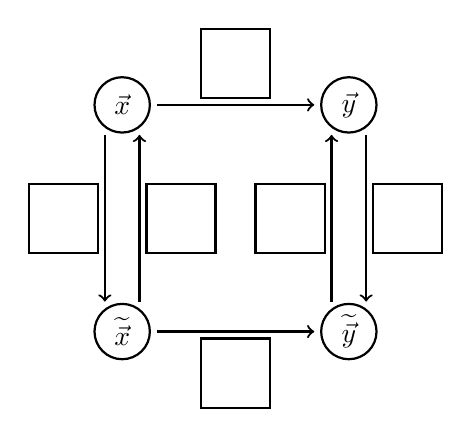
\begin{tikzpicture}[node distance = 2cm, thick, every node/.style={inner sep=0.25em,outer sep=0.25em}]%
      \node (1) [circle,draw,minimum size=2em] {$\vec{x}$};
      \node (2) [circle,draw,right=of 1,minimum size=2em] {$\vec{y}$};
      \node (3) [circle,draw,below=of 2,minimum size=2em] {$\widetilde{\vec{y}}$};
      \node (4) [circle,draw,below=of 1,minimum size=2em] {$\widetilde{\vec{x}}$};
      \draw[->] (1) -- node [rectangle,draw,midway,above,minimum size=2.5em] {} (2);
      \draw[->] (1.240) -- node [rectangle,draw,midway,left,minimum size=2.5em]{} (4.120);
      \draw[->] (4.60) -- node [rectangle,draw,midway,right,minimum size=2.5em]{} (1.300);
      \draw[->] (2.300) -- node [rectangle,draw,midway,right,minimum size=2.5em]{} (3.60);
      \draw[->] (3.120) -- node [rectangle,draw,midway,left,minimum size=2.5em]{} (2.240);
      \draw[->] (4) -- node [rectangle,draw,midway,below,minimum size=2.5em] {} (3);
    \end{tikzpicture}%
  \end{figure}
}

\sol {
  \begin{figure}[H]
    \centering
    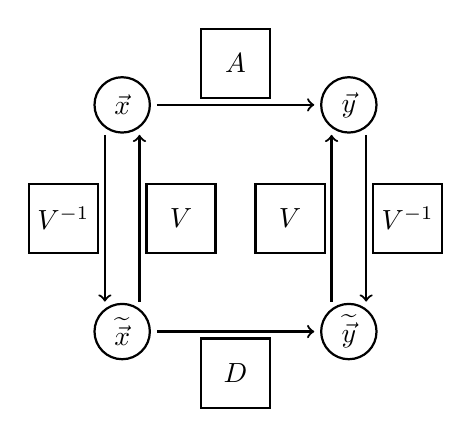
\begin{tikzpicture}[node distance = 2cm, thick, every node/.style={inner sep=0.25em,outer sep=0.25em}]%
      \node (1) [circle,draw,minimum size=2em] {$\vec{x}$};
      \node (2) [circle,draw,right=of 1,minimum size=2em] {$\vec{y}$};
      \node (3) [circle,draw,below=of 2,minimum size=2em] {$\widetilde{\vec{y}}$};
      \node (4) [circle,draw,below=of 1,minimum size=2em] {$\widetilde{\vec{x}}$};
      \draw[->] (1) -- node [rectangle,draw,midway,above,minimum size=2.5em] {$A$} (2);
      \draw[->] (1.240) -- node [rectangle,draw,midway,left,minimum size=2.5em]{$V^{-1}$} (4.120);
      \draw[->] (4.60) -- node [rectangle,draw,midway,right,minimum size=2.5em]{$V$} (1.300);
      \draw[->] (2.300) -- node [rectangle,draw,midway,right,minimum size=2.5em]{$V^{-1}$} (3.60);
      \draw[->] (3.120) -- node [rectangle,draw,midway,left,minimum size=2.5em]{$V$} (2.240);
      \draw[->] (4) -- node [rectangle,draw,midway,below,minimum size=2.5em] {$D$} (3);
    \end{tikzpicture}%
  \end{figure}

  You can explain $A = VDV^{-1}$ by just left-multiplying in the order of the arrows from $\vec{x}$ to $\vec{y}$. Again, in the change of basis perspective, $V^{-1}$ first pulls the vector $\vec{x}$ into the eigenbasis. $D$ performs the equivalent linear transformation of $A$ but in the eigen-coordinate system. Finally, $V$ brings the transformed vector back into standard coordinates.
}

\end{enumerate}

\newpage
\input{\bank/vector-diff-eq/vector_diff_eq}
\end{qunlist}

\end{document}
